\subsection{Pharmacokinetics} \label{PKPD}

In this section, I describe pharmacokinetics as it will be used in the proposed research.  I will explain aspects of both pharmacokinetic and pharmacodynamic models, and how the two are related.  One-- and two-- compartment model(s) for pharmacokinetics will be constructed and interpreted.


\subsubsection{A One Compartment Pharmacokinetic Model} 

To analyze the time course of drug mass in various parts of the body, compartmental models may be used.  These models posit that the body (or relevant organs/systems of the body) is comprised of compartments from which drug can flow in and out. The rates at which the drug can enter and exit each compartment are specified, and a differential equation for each compartment can be written down and solved using methods outlined in \cref{sec:ODE}.

An example of these models used for orally-administered drugs is the one--compartment pharmacokinetic model with first order elimination.  The model posits the following \cite{wakefield1992bayesian}:  
%
\begin{itemize}
\item The rate of drug absorption from the gut ($ G  $) into the blood plasma ($ C $) is proportional to the amount of drug in the gut and that is the proportionality constant is $ k_a $, in units $ \text{hours}^{-1} $;

\item The rate of elimination from the blood plasma is proportional to the amount of drug in the plasma compartment with proportionality constant $ k $, in units $ \text{hours}^{-1} $;

\item The volume of plasma in the body is $ V $, in units litres;

\item The bioavailability of the drug (i.e. the fraction of drug absorbed into the blood serum) is $F$;
\end{itemize}
%
 A visual representation of this model is shown in \cref{compartmental_model}.

\begin{figure}[h!]
	\centering
	
	\tikzstyle{int}=[draw, fill=white, minimum size=2em]
	\tikzstyle{init} = [pin edge={to-,thin,black}]
	
	
	\begin{tikzpicture}[node distance=2.5cm,auto,>=latex']
	
	
	\node [int] (a) {$G$};
	\node (b) [left of=a,node distance=2cm, coordinate] {a};
	\node [int] (c) [right of=a] {$C$};
	\node [coordinate] (end) [right of=c, node distance=2cm]{};
	\path[->] (a) edge node {$k_a$} (c);
	\draw[->] (c) edge node {$k$} (end) ;
	\end{tikzpicture}
	\caption[Pharmacokinetic compartmental diagram]{A compartmental diagram for a one compartment pharmacokinetic model.  Arrows indicate the direction of flux.  Flux is proportional to the concentration in each compartment, with rate constants indicated over the arrows.}
	\label{compartmental_model}
\end{figure}

The pharmacokinetic model described in \cref{compartmental_model} can be written as a system of differential equations.  Let $D$ be the size of the oral dose (in units of mass).  The differential equations are then
%
\begin{alignat*}{3}
	\dfrac{dG}{dt} &= -k_aG \>, \quad  &&G(0) = D \\
	\dfrac{dC}{dt} &= k_aG - kC \>,   \quad  &&C(0) = 0
\end{alignat*}
%
 
 The differential equation for $dG/dt$ can be solved to yield $G(t) = D\exp(-k_a t)$.  The differential equation governing the mass transit if drug in/out of the $C$ compartment is then $dC/dt = k_aD\exp(-k_a t) - kC$.  This differential equation can be solved analytically.  The concentration of the drug in the $C$ compartment can be obtained by dividing $C(t)$ by the volume of the $C$ compartment, $V$.  The solution for $C(t)$ after converting to a concentration is 

\begin{equation}\label{onecompartment_PKPD}
	C(t) = \dfrac{F\times D}{V}\dfrac{k_a}{k - k_a}\Big(e^{-k_at} - e^{-kt}\Big) \>.
\end{equation}

\noindent The qualitative behaviour of \cref{onecompartment_PKPD} can be examined for families of similar parametrizations through non-dimensionalization. Let $\tau$ and $y(\tau)$ be dimensionless quantities.  By letting $C(t) = k_a D/V y(t\tau)$ and $t = \tau/k_a$, the non-dimensional solution to the differential equation governing mass transit of the drug is 

\begin{equation}\label{non_dim_eqn}
	y(\tau) = \dfrac{1}{\alpha-1} \Big(  \exp(-t) - \exp(-\alpha t) \Big)
\end{equation}

\noindent Here, $ \alpha = k/k_a $ is the ratio of the elimination and absorption rate constants.  Shown in \cref{fig:pkcureves} is \cref{non_dim_eqn} under different parametrizations of $\alpha$.  

\begin{figure}[h!]
	\centering
	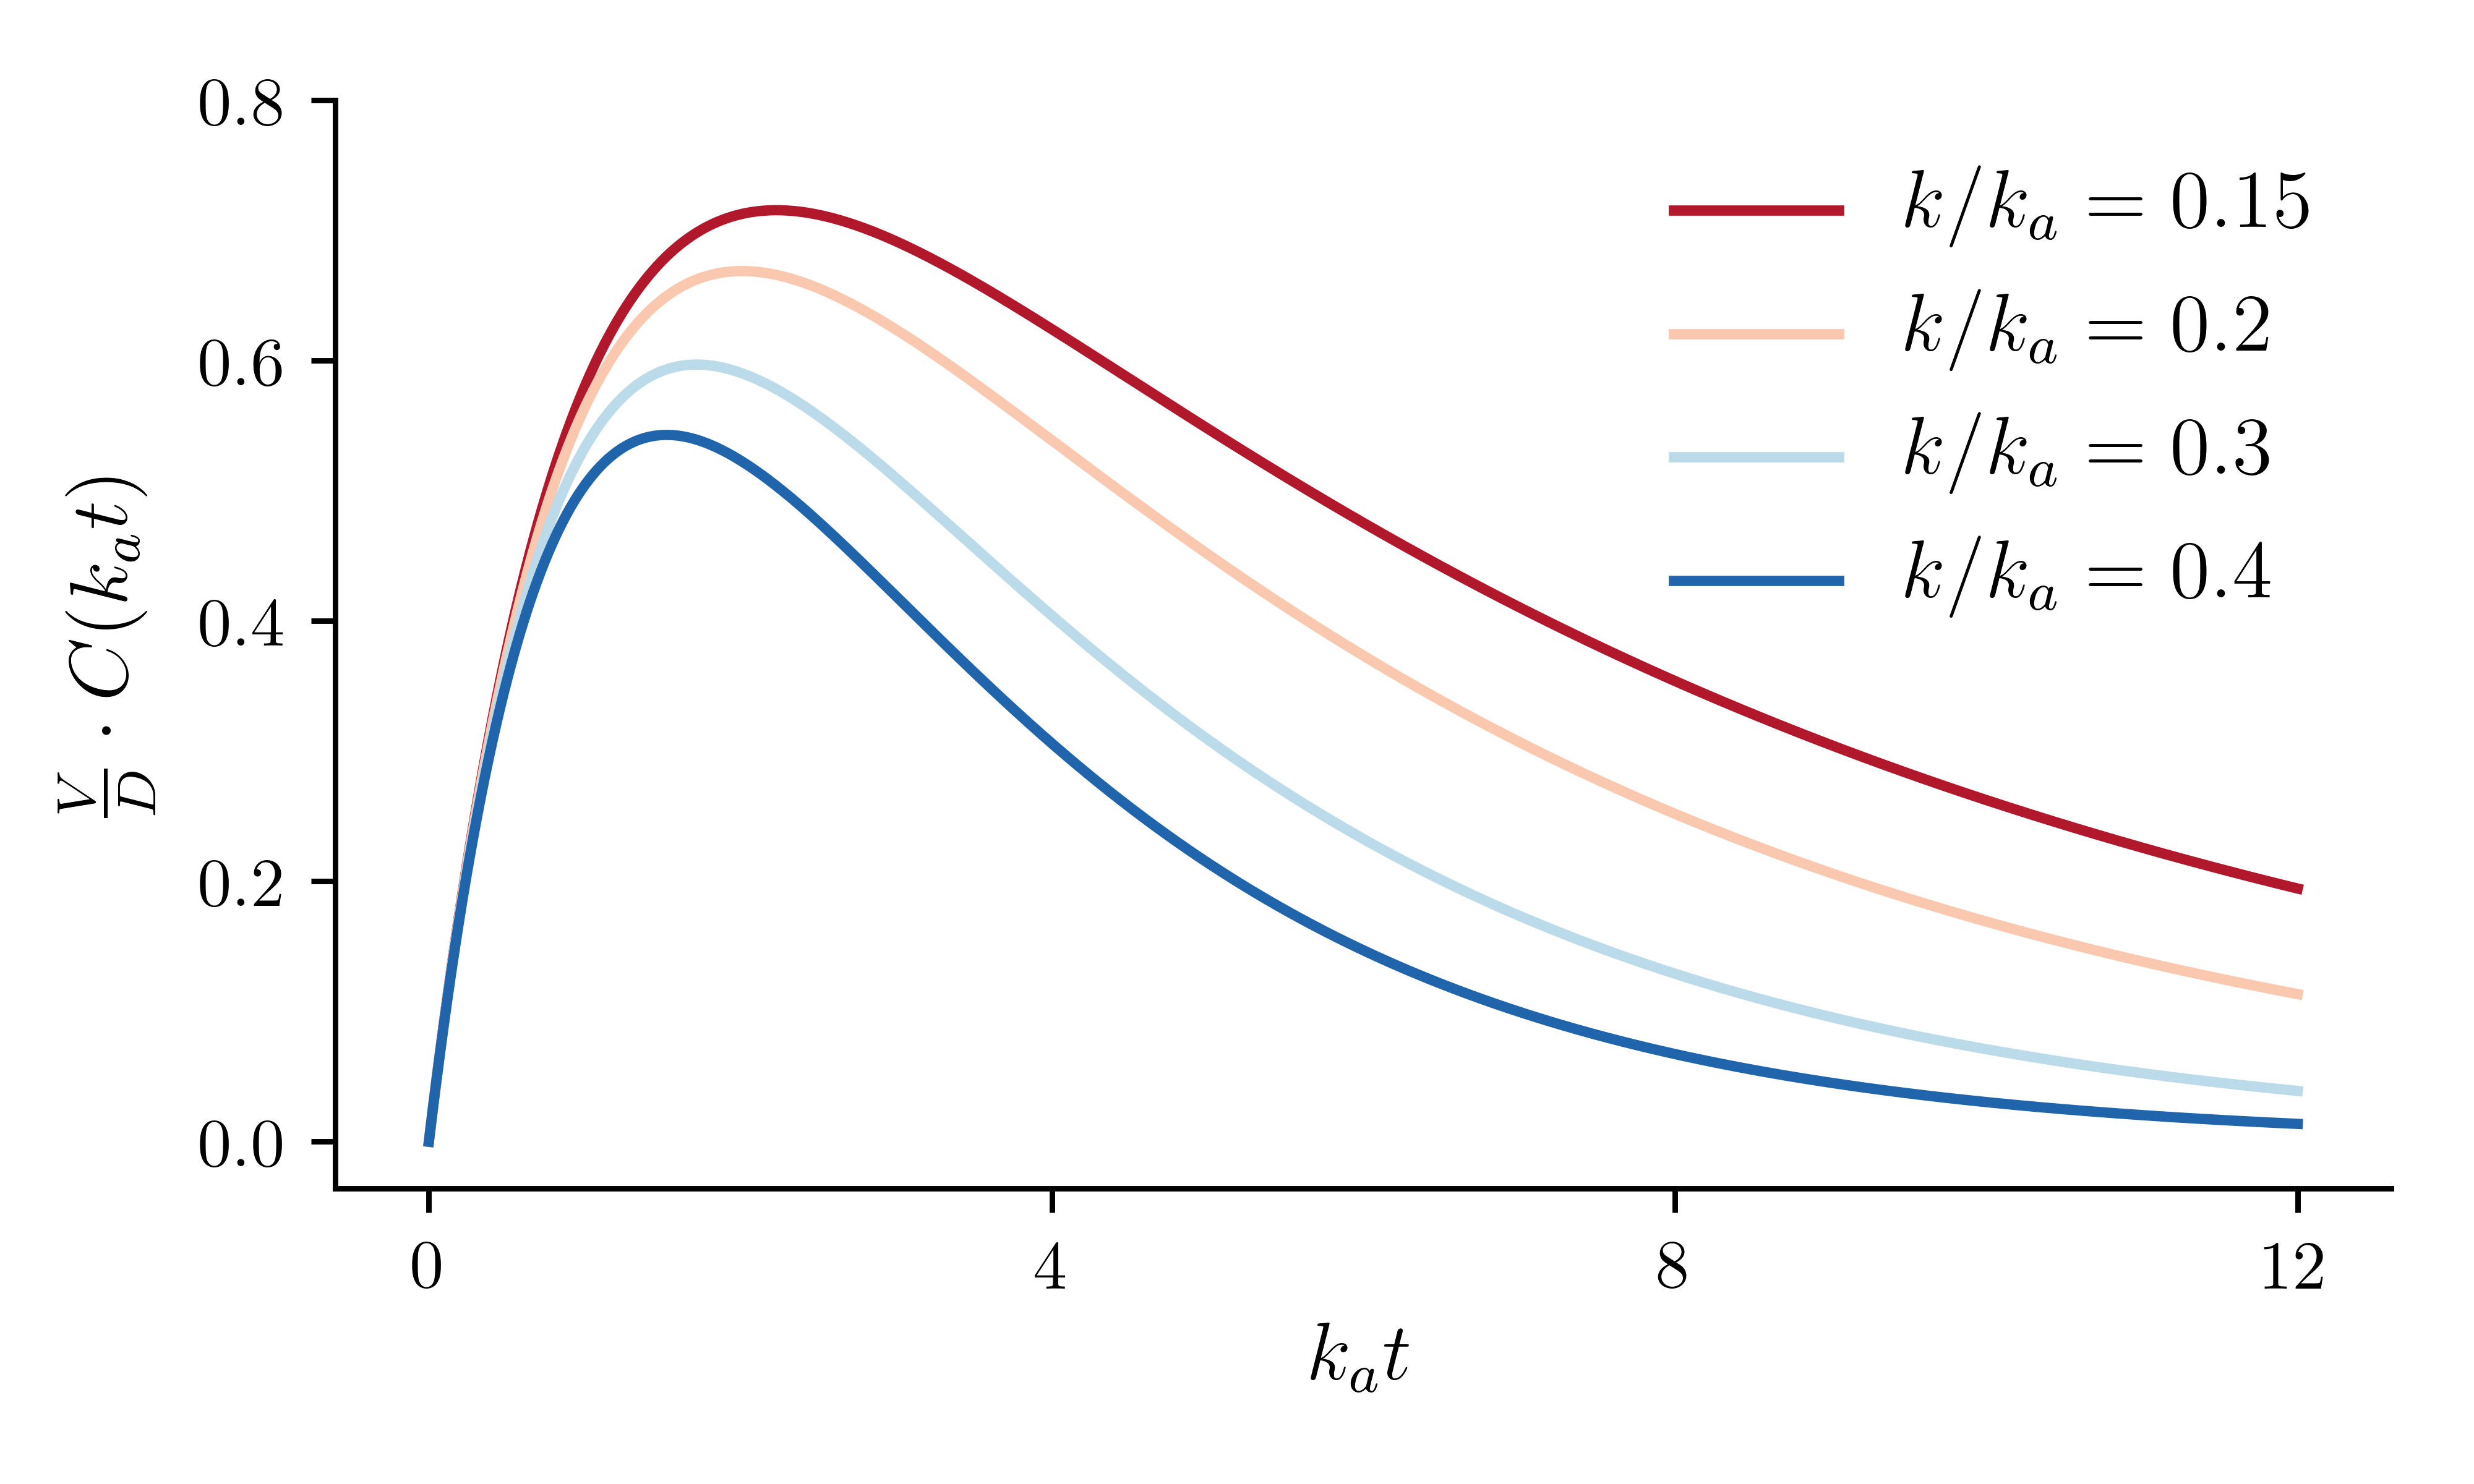
\includegraphics{figures/pkcurves.png}
	\caption[Non-dimensionalized solutions to pharmacokinetic differential equation] {Non-dimensionalized concentration plotted against non-dimensionalized time.  The process non-dimensionalizing the differential equation removes all units from the model, allowing for qualitative comparisons of the solution under different families of parameterization.  Here, it is shown that all parametrizations in which $\alpha = k/ka = 0.15$ elicit larger concentrations than those parameterizations in which $\alpha=0.4$ conditioned on $V/D$ remaining constant.}
	\label{fig:pkcureves}
\end{figure}


\subsubsection{A Two Compartment Pharmacokinetic Model}

The model presented above can be extended to include a second compartment, $C_2$ which may be the concentration of the drug at its site of action.  The assumptions for the previous models still hold, but now the model allows for flux of drug between the blood serum compartment and site of action compartment, as well as elimination of the drug from both compartments. Shown in \cref{two_compartmental_model} is a compartmental diagram for the two compartment pharmacokinetic model.

\begin{figure}[h!]
	\centering
	
	\tikzstyle{int}=[draw, fill=white, minimum size=2em]
	\tikzstyle{init} = [pin edge={to-,thin,black}]
	
	
	\begin{tikzpicture}[node distance=2.5cm,auto,>=latex']
	
	\node [int] (G){$G$};
	\node [int] (C1)[right of = G]{$C_1$};
	\node [int] (C2)[right of = C1]{$C_2$};
	
	\node [coordinate] (C1_exit) [below of=C1, node distance=2cm]{};
	 
	 \path[->](G) edge node {$k_a$} (C1);
	 \path[->, bend left](C1) edge node {$k_{12}$} (C2);
	 \path[<-, bend right](C1) edge node {$k_{21}$} (C2);
	 \path[->](C1) edge node {$k_1$} (C1_exit);

	\end{tikzpicture}
	\caption{Two compartment pharmacokinetic model.}
	\label{two_compartmental_model}
\end{figure}

The differential equations governing this system are

\begin{alignat*}{3}
\dfrac{dG}{dt} &= -k_aG \>, \quad  &&G(0) = D \\
\dfrac{dC_1}{dt} &= k_aG + k_{21}C_2 - (k_1  + k_{12})C_1 \>,   \quad  &&C_1(0) = 0\\
\dfrac{dC_2}{dt} &= k_{12}C_1 - (k_{21})C_2\>,   \quad  &&C_2(0) = 0
\end{alignat*}

These models are easily constructed to arbitrarily many compartments, but with more compartments comes a need for data from those compartments, which may not always be feasible.

